%!TEX root = ../main.tex

% TODO box delle sintassi
% TODO box della semantica finale
% TODO parentesi nelle condizioni
% TODO ricontrollare le sintassi che siano uguali
% TODO traduzione codice: copiare direttamente da xtext?
% TODO acronimi: invertire la prima comparsa
% TODO citazione a inizio capitolo: LAPSA -> volpe in léttone

\myChapter{LAPSA}

Per definire ed implementare un modello di un sistema adattivo possono essere utilizzati molti strumenti già esistenti. L'approccio che vogliamo impiegare coinvolge l'utilizzo di un model checker come supporto alle scelte che possiamo semplicemente scegliere a seconda delle specifiche e delle esigenze dello scenario.

Prendiamo come punto di riferimento, quindi, l'unico elemento sicuro che abbiamo a disposizione: l'agente principale, cioè quello per il quale deve essere trovata una strategia che lo porti al suo obiettivo. Quello che ci si può immaginare è che questo agente proceda in parallelo con la parte che non conosce: l'ambiente (figura \ref{fig:lapsa:schemaidea}). L'ambiente può essere costituito da più agenti o altri tipi di sistemi di cui si può avere una conoscenza solamente parziale o nulla.
\begin{figure}[htbp!]
	\begin{center}
		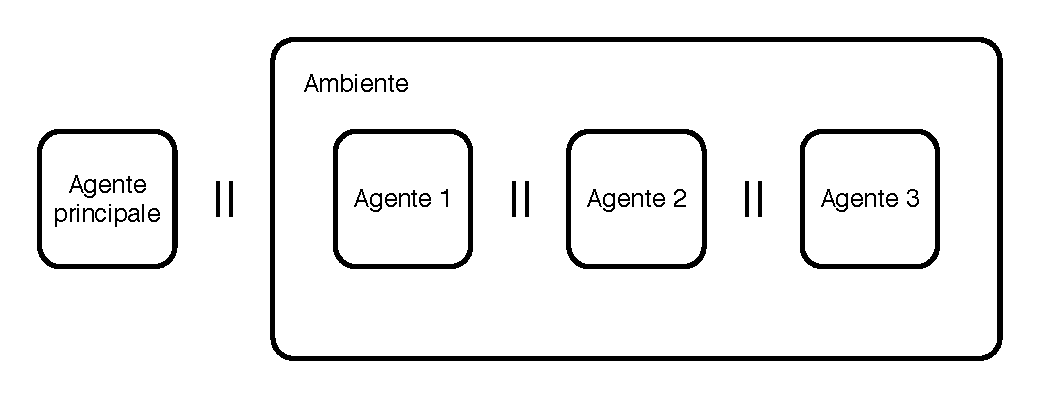
\includegraphics[width=.8\textwidth]{Images/schemaidea}
	\end{center}
	\caption{Schema di come viene modellato uno scenario attorno all'agente che lo analizza}
	\label{fig:lapsa:schemaidea}
\end{figure}

L'approccio che vogliamo utilizzare è quello di \emph{formulare un'ipotesi} sulla composizione ed il comportamento dell'ambiente ed utilizzare il model checker su questo modello verificando la formula che rappresenta l'obiettivo dell'agente principale. Cambiamo quindi la prospettiva classica del model checking fornendo un modello ipotetico per fare \emph{previsioni}. Quello che vogliamo che l'agente finale abbia alla fine di questo procedimento è una valutazione quantitativa di quanto ogni scelta ha la possibilità di portarlo al raggiungimento dell'obiettivo.

In questo capitolo viene introdotta la definizione del linguaggio \ac{lapsa}, un linguaggio specifico per agenti adattivi. L'obiettivo che si vuole raggiungere con questo linguaggio è definire un'interfaccia che permetta di modellare sistemi adattivi in modo più efficiente ed efficace possibile. Si parla di interfaccia in quanto, attraverso la definizione di sintassi e semantica, si dichiara \emph{cosa} possono fare i costrutti linguistici di \ac{lapsa} (front-end) senza entrare in merito del \emph{come} questo verrà implementato (back-end).

Il back-end è stato implementato in \java{} tramite \xtext{} \cite{xtext}, un meta-tool specifico per la creazione di plugin \eclipse{} di linguaggi personalizzati. Definendo la grammatica del proprio linguaggio è possibile implementarne velocemente la traduzione del codice ed i servizi di utilità più diffusi come l'autocompletamento e la colorazione delle parole chiave. Oltre al compilatore è presente anche il model checker \prism{} in grado di eseguire i controlli di formule \ac{pctl} su \ac{mdp} definite secondo il suo specifico linguaggio.

L'approccio utilizzato separa il linguaggio dal livello implementativo permettendo di cambiare gli strumenti sottostanti senza che l'utilizzatore debba venirne a conoscenza, a patto che i nuovi strumenti rispettino la semantica dei costrutti linguistici.

\section{Sintassi}
Per descrivere la sintassi \ac{lapsa} sarà utilizzato il formalismo \emph{EBNF} indicando con le parole in corsivo i simboli non terminali e con quelle in neretto e quelle in stampatello i non terminali. Le parole in neretto sono \emph{keyword} del linguaggio mentre quelle in stampatello descrivono dei valori arbitrari su insiemi come nomi di variabili o costanti numeriche. Procederemo con la descrizione informale di cosa viene identificato con i costrutti sintattici del linguaggio introducendoli gradualmente.

Il non terminale \emph{program} è il simbolo iniziale della grammatica e nella sua struttura racchiude la dichiarazione dell'insieme di azioni considerato, il modulo che descrive il comportamento del soggetto, i moduli che possono essere usati per descrivere l'ambiente e i dati necessari alla discretizzazione delle variabili (tabella \ref{tab:lapsaProgram}).

\begin{table}[htbp!] % sintassi programma LAPSA
$$
\begin{array}{rcl}
	\mathit{program} &::=& \mathbf{actions} \Space \{ \mathit{actions} \} \\
		&& \mathbf{subject} \Space \mathit{module} \\
		&& \mathit{modules} \\
		&& \mathit{environment} \\
		&& \mathbf{ranges} \Space \{ \mathit{ranges} \} \\
\end{array}
$$
\caption{Sintassi \ac{lapsa} di \emph{program}}
\label{tab:lapsaProgram}
\end{table}

Il non terminale \emph{actions} è una semplice lista dove vengono dichiarate i nomi delle azioni che possono essere effettuate (tabella \ref{tab:lapsaActions}). Ovviamente le azioni utilizzate in seguito nelle transizioni dei moduli e nelle sincronizzazioni dovranno essere state dichiarate in questa sezione per considerare il programma \emph{corretto}.

\begin{table}[htbp!] % sintassi azioni LAPS
$$
\begin{array}{rcl}
	\mathit{actions} &::=& \x{action}\textrm{-}\x{id} \Sep \mathit{actions} \Space \mathit{actions} \\
\end{array}
$$
\caption{Sintassi \ac{lapsa} di \emph{actions}}
\label{tab:lapsaActions}
\end{table}

La definizione di un comportamento viene espressa tramite il non terminale \emph{module} che permette di descrivere i suoi dati, le sue transizioni e i suoi obiettivi (tabella \ref{tab:lapsaModule}). I dati sono rappresentati dalla lista \emph{variables} e ogni dato è rappresentato dal tipo di dato, il nome associato e l'espressione che gli attribuisce un valore iniziale. Con il non terminale \emph{rules}, invece, viene descritta una lista di transizioni. Le transizioni vengono definite come la tripla \emph{condizione}, \emph{azione}, \emph{distribuzione}: se la condizione è vera allora può essere effettuata l'azione e l'aggiornamento dello stato secondo la distribuzione di probabilità. Gli obiettivi vengono descritti nella lista \emph{targets} dove il primo criterio ha importanza massima e decrementa fino all'ultimo che sarà il meno importante.

\begin{table}[htbp!] % sintassi modulo LAPSA
$$
\begin{array}{rcl}
	\mathit{module} &::=& \mathbf{module} \Space \x{module}\textrm{-}\x{id} \Space \{ \mathit{variables} \Space \mathit{rules} \Space \mathit{targets} \}
		\\[.3cm]
	\mathit{variables} &::=& \x{type} \Space \x{variable}\textrm{-}\x{id} = \mathit{expression}; \Sep \mathit{variables} \Space \mathit{variables}
		\\[.3cm]
	\mathit{rules} &::=& \mathit{condition} [ \x{action}\textrm{-}\x{id}] \Rightarrow \mathit{distribution}; \Sep \mathit{rules} \Space \mathit{rules}
		\\[.3cm]
	\mathit{targets} &::=& \mathbf{target} \Space \mathbf{never} \Space \mathit{condition} \Sep \mathit{targets} \Space \mathit{targets} \\
\end{array}
$$
\caption{Sintassi \ac{lapsa} di \emph{module} e delle sezioni che lo compongono}
\label{tab:lapsaModule}
\end{table}

Le distribuzioni di probabilità (tabella \ref{tab:lapsaDistribution}) sono definite come un insieme di possibili aggiornamenti dello stato associati ad un certo valore di probabilità. Questo valore viene espresso nel costrutto sintattico dall'espressione all'interno delle parentesi angolate e viene normalizzato con gli altri nel caso in cui la somma non sia $1$. Questi valori possono anche dipendere dalle variabili di stato e quindi variare con l'avanzamento del modello.

\begin{table}[htbp!] % sintassi delle distribuzioni in LAPSA
$$
\begin{array}{rcl}
	\mathit{distribution} &::=& <\mathit{expression}> \mathit{update} \Sep \mathit{distribution} \Space \# \Space \mathit{distribution} \\
\end{array}
$$
\caption{Sintassi \ac{lapsa} di \emph{distribution}}
\label{tab:lapsaDistribution}
\end{table}

Ogni caso di una distribuzione porta a una lista di aggiornamenti che possono essere descritti con i costrutti sintattici definiti in tabella \ref{tab:lapsaUpdate}. Si può modificare il valore di una variabile tramite assegnamento o specificare che nessun cambiamento verrà eseguito tramite l'operazione nulla \texttt{noaction}. Per mezzo degli operatori \texttt{env.add} e \texttt{env.remove} è possibile agire sull'ambiente aggiungendo e rimuovendo elementi rispettivamente.

\begin{table}[htbp!] % sintassi degli aggiornamenti in LAPSA
$$
\begin{array}{rcl}
	\mathit{update} &::=& \x{variable}\textrm{-}\x{id} = \mathit{expression} \Sep \mathbf{noaction} \\
		& \Sep & \mathit{update} \Space , \Space \mathit{update} \\
\end{array}
$$
\caption{Sintassi \ac{lapsa} di \emph{update}}
\label{tab:lapsaUpdate}
\end{table}

Il non terminale \emph{modules} descritto, assieme ad \emph{environment}, in tabella \ref{tab:lapsaModules} viene utilizzato per definire un insieme di moduli che poi potranno essere istanziati nell'ambiente con dei riferimenti al loro nome. Questo accade all'interno del non terminale \emph{environment} dove viene descritto l'ambiente come una lista di riferimenti a moduli intervallati dagli insiemi di azioni su cui possono sincronizzarsi, un operatore che riprende sintatticamente e semanticamente dal parallelo di Hoare in \ac{csp} \cite{Hoare:1978:CSP}.

\begin{table}[htbp!] % sintassi della definizione dei moduli e dell'ambiente in LAPSA
$$
\begin{array}{rcl}
	\mathit{modules} &::=& \mathit{module} \Sep \mathit{modules} \Space \mathit{modules}
		\\[.3cm]
	\mathit{environment} &::=& \x{module}\textrm{-}\x{id} \Sep \mathit{environment} \Par{\{\mathit{actions}\}} \mathit{environment}
		\\
\end{array}
$$
\caption{Sintassi \ac{lapsa} di \emph{modules} e di \emph{environment}}
\label{tab:lapsaModules}
\end{table}

Le condizioni hanno un ruolo importante in quanto parte fondamentale dell'abilitazione delle transizioni. La sintassi di una condizione è illustrata in tabella \ref{tab:lapsaCondition} e mette a disposizione, oltre ai costrutti sintattici più classici come gli operatori booleani e il confronto tra espressioni, anche il quantificatore esistenziale. Questo operatore viene considerato soddisfatto se esiste un modulo del tipo specificato che soddisfa la condizione espressa. La condizione del quantificatore esistenziale può fare riferimento al nome temporaneo associato al tipo di modulo interessato in modo da poter indagare sulle sue variabili di stato.

\begin{table}[htbp!] % sintassi delle condizioni in LAPSA
$$
\begin{array}{rcl}
	\mathit{condition} &::=& \mathbf{exists} \Space \x{variable}\textrm{-}\x{id}:\x{module}\textrm{-}\x{id} \Space \mathbf{such}\Space\mathbf{that} \Space \mathit{condition} \\
		& \Sep & \mathit{expression} \bowtie \mathit{expression} \Sep \mathbf{true} \\
		& \Sep & \mathit{condition} \Space \mathbf{or} \Space \mathit{condition} \Sep \mathbf{not} \Space \mathit{condition}
		\\
\end{array}
$$
\caption{Sintassi \ac{lapsa} di \emph{condition}}
\label{tab:lapsaCondition}
\end{table}

Il simbolo $\bowtie$ rappresenta l'operatore di confronto e può essere quindi definito come $\bowtie = \{<,\leq,>,\geq, =, \neq\}$. Le espressioni (tabella \ref{tab:lapsaExpression}) sono fondamentalmente variabili e costanti numeriche combinate tra loro tramite i classici operatori binari e gli operatori di confronto seguono l'interpretazione classica.
Le variabili referenziate devono essere precedute dall'istanza di appartenenza: se fanno riferimento al modulo nel quale vengono richiamate si utilizza la keyword \texttt{this}, altrimenti il riferimento al modulo interessato nel caso in cui si stia esprimendo una condizione interna ad un quantificatore esistenziale.

\begin{table}[htbp!] % sintassi delle espressioni in LAPSA
$$
\begin{array}{rcl}
	\mathit{expression} &::=& \mathit{expression} \Space \mathit{bop} \Space \mathit{expression} \Sep \mathit{reference} \\
	& \Sep & (\mathit{expression}) \Sep \x{constant}
	\\[.3cm]
	\mathit{reference} &::=& (\x{variable}\textrm{-}\x{id} \Sep \mathbf{this})\mathbf{.} \x{variable}\textrm{-}\x{id}
	\\[.3cm]
	\mathit{bop} &::=& + \Sep - \Sep * \Sep \slash
	\\
\end{array}
$$
\caption{Sintassi \ac{lapsa} di \emph{expression}}
\label{tab:lapsaExpression}
\end{table}

Infine il non terminale \emph{ranges} (tabella \ref{tab:lapsaRanges}) permette di descrivere i range di tutte le variabili dei moduli. Questo costrutto è stato inserito in aggiunta alla normale interfaccia di \ac{lapsa} per adattarne l'implementazione del backend a \prism{} che necessita la conoscenza dei possibili valori delle variabili.

In tabella \ref{tab:lapsaSyntax} viene riportata la sintassi completa di \ac{lapsa} i cui costrutti possono essere estesi 

\begin{table}[htbp!] % sintassi dei range in LAPSA
$$
\begin{array}{rcl}
	\mathit{ranges} &::=& \mathit{reference} \Space \mathbf{in} [\x{constant}, \x{constant}] \Sep \mathit{ranges}, \mathit{ranges} \\
\end{array}
$$
\caption{Sintassi \ac{lapsa} di \emph{ranges}}
\label{tab:lapsaRanges}
\end{table}

\begin{table}[htbp!] % sintassi completa LAPSA
$$
	\begin{array}{|rcl|}
	\hline
	\mathit{program} &::=& \mathbf{actions} \Space \{ \mathit{actions} \} \\
		&& \mathbf{subject} \Space \mathit{module} \\
		&& \mathit{modules} \\
		&& \mathit{environment} \\
		&& \mathbf{ranges} \Space \{ \mathit{ranges} \} 
	\\[.3cm]
	\mathit{actions} &::=& \x{action}\textrm{-}\x{id} \Sep \mathit{actions} \Space \mathit{actions} 
	\\[.3cm]
	\mathit{module} &::=& \mathbf{module} \Space \x{module}\textrm{-}\x{id} \Space \{ \mathit{variables} \Space \mathit{rules} \Space \mathit{targets} \}
	\\[.3cm]
	\mathit{variables} &::=& \x{type} \Space \x{variable}\textrm{-}\x{id} = \mathit{expression}; \Sep \mathit{variables} \Space \mathit{variables}
	\\[.3cm]
	\mathit{rules} &::=& \mathit{condition} [ \x{action}\textrm{-}\x{id}] \Rightarrow \mathit{distribution}; \Sep \mathit{rules} \Space \mathit{rules}
	\\[.3cm]
	\mathit{targets} &::=& \mathbf{target} \Space \mathbf{never} \Space \mathit{condition} \Sep \mathit{targets} \Space \mathit{targets} 
	\\[.3cm]
	\mathit{distribution} &::=& <\mathit{expression}> \mathit{update} \Sep \mathit{distribution} \Space \# \Space \mathit{distribution} 
	\\[.3cm]
	\mathit{update} &::=& \x{variable}\textrm{-}\x{id} = \mathit{expression} \Sep \mathbf{noaction} \\
		& \Sep & \mathit{update} \Space , \Space \mathit{update} 
	\\[.3cm]
	\mathit{modules} &::=& \mathit{module} \Sep \mathit{modules} \Space \mathit{modules}
	\\[.3cm]
	\mathit{environment} &::=& \x{module}\textrm{-}\x{id} \Sep \mathit{environment} \Par{\{\mathit{actions}\}} \mathit{environment}
	\\[.3cm]
	\mathit{condition} &::=& \mathbf{exists} \Space \x{variable}\textrm{-}\x{id}:\x{module}\textrm{-}\x{id} \Space \mathbf{such}\Space\mathbf{that} \Space \mathit{condition} \\
		& \Sep & \mathit{expression} \bowtie \mathit{expression} \Sep \mathbf{true} \\
		& \Sep & \mathit{condition} \Space \mathbf{or} \Space \mathit{condition} \Sep \mathbf{not} \Space \mathit{condition}
	\\[.3cm]
	\mathit{expression} &::=& \mathit{expression} \Space \mathit{bop} \Space \mathit{expression} \Sep \mathit{reference} \\
	& \Sep & (\mathit{expression}) \Sep \x{constant}
	\\[.3cm]
	\mathit{reference} &::=& \x{variable}\textrm{-}\x{id}\mathbf{.}\x{variable}\textrm{-}\x{id} \Sep \mathbf{this}\mathbf{.}\x{variable}\textrm{-}\x{id}
	\\[.3cm]
	\mathit{bop} &::=& + \Sep - \Sep * \Sep \slash
	\\[.3cm]
	\mathit{ranges} &::=& \x{module}\textrm{-}\x{id}\mathbf{.}\x{variable}\textrm{-}\x{id} \Space \mathbf{in} [\x{constant}, \x{constant}] \Sep \mathit{ranges}, \mathit{ranges} 
	\\
	\hline
	\end{array}
$$
\caption{Sintassi di \ac{lapsa}}
\label{tab:lapsaSyntax}
\end{table}

\section{Zucchero sintattico}
La sintassi presentata in tabella \ref{tab:lapsaSyntax} è concreta ma contiene solo gli operatori primitivi ed è dunque solo il nucleo del linguaggio che si vuole utilizzare. Al fine di aumentare la semplicità di comprensione e di scrittura del linguaggio \ac{lapsa} intrudiciamo alcuni costrutti di utilità come una rielaborazione di quelli primitivi già presenti.

Con gli operatori logici possiamo ridefinire i seguenti costrutti all'interno del non terminale \emph{condition}, assumendo $\alpha$ come un $\x{variable}\textrm{-}\x{id}$, $\gamma$ come un $\x{module}\textrm{-}\x{id}$ e $\beta,\beta' \in \mathit{condition}$
$$
\begin{array}{l}
	\mathbf{false} \equiv \mathbf{not} \Space \mathbf{true}
	\\[.3cm]
	\beta \Space \mathbf{and} \Space \beta' \equiv \mathbf{not} \Space (\mathbf{not} \Space \beta \Space \mathbf{or} \Space \mathbf{not} \Space \beta')
	\\[.3cm]
	\mathbf{forall} \Space \alpha:\gamma \Space \mathbf{such} \Space \mathbf{that} \Space \beta \equiv \mathbf{not} \Space \mathbf{exists} \Space \alpha:\gamma \Space \mathbf{such} \Space \mathbf{that} \Space \mathbf{not} \Space \beta
	\\
\end{array}
$$

Inseriamo un costrutto di \emph{rule} tale da poter inserire una condizione di abilitazione dei singoli casi delle distribuzioni, assumendo $\alpha$ come un $\x{action}\textrm{-}\x{id}$, $\beta, \beta' \in \emph{condition}$, $\delta \in \mathit{distribution}$ ed $\epsilon \in \mathit{expression}$
$$
\beta [\alpha] \Rightarrow <\epsilon,\beta'> \alpha \Space \# \Space \delta
\equiv
\beta \Space \mathbf{and} \Space \beta' [\alpha]\Rightarrow <\epsilon> \alpha \Space \# \Space \delta,
\beta \Space \mathbf{and} \Space \mathbf{not} \Space \beta' [\alpha]\Rightarrow \delta
$$

Dato che in \ac{lapsa} è presente il non determinismo se più guardie sono abilitate allo stesso passo, introduciamo la possibilità di scrivere più distribuzioni con una sola guardia che vale per tutte le regole. Sia $\alpha$ un $\x{action}\textrm{-}\x{id}$, $\beta \in \mathit{condition}$ e $\delta,\delta' \in \mathit{distribution}$, introduciamo il seguente costrutto del non terminale \emph{rule}
$$
\beta [\alpha] \Rightarrow \delta \Rightarrow \delta';
\equiv
\beta [\alpha] \Rightarrow \delta; \beta [\alpha] \Rightarrow \delta'; 
$$

Possiamo ottenere con facilmente il costrutto che esprime un obiettivo che vogliamo mantenere durante tutta l'esecuzione:
$$
	\mathbf{target}\ \mathbf{always}\ \mathit{condition} \equiv \mathbf{target}\ \mathbf{never}\ \mathbf{not}\ \mathit{condition}
$$

Infine, per quanto riguarda i riferimenti a variabile, è possibile assumere in assenza del prefisso di appartenenza che la variabile appartenga al modulo locale di default:
$$
	\x{variable}\textrm{-}\x{id} \equiv \mathbf{this}.\x{variable}\textrm{-}\x{id}
$$

%------------------------------------------------------------------------------------
% SEMANTICA
%------------------------------------------------------------------------------------
\section{Semantica}
Durante la descrizione della sintassi sono stati presentati informalmente i costrutti di \ac{lapsa}, passiamo adesso a dare una definizione formale della loro semantica. Rappresenteremo il significato di un programma \ac{lapsa} tramite una \ac{mdp} perché permette di esprimere le transizioni tra stati come scelte nondeterministiche di distrubuzioni di probabilità aventi come supporto l'insieme degli stati stessi.

Ad ogni nonterminale \emph{module} sarà associata una \ac{mdp} della forma
$$ M = (\Sigma,Act,\rightarrow_\rho,\sigma_0) $$
Le parti che compongono la \ac{mdp} sono descritte in seguto, tenendo conto che ogni riferimento ai nodi della sintassi viene inteso come appartenente al modulo in questione e, per semplicità, utilizziamo la notazione $eval(e)$ con $e \in \mathit{expression}$ per indicare la valutazione di un'espressione nel modo classico. 
\begin{itemize}
	\item $\Sigma = \{\sigma \sep \sigma : \mathbb{VAR} \rightarrow \mathbb{VAL}\}$ è l'insieme degli \emph{stati} rappresentati da funzioni che mappano variabili in valori, dove $\mathbb{VAR}$ è l'insieme delle $\x{variable}\textrm{-}\x{id}$ definite nel modulo e $\mathbb{VAL} \subset \mathbb{N}_0$ di cardinalità finita
	\item $\sigma_0 \in \Sigma$ è lo \emph{stato iniziale} del modulo ottenuto tramite la valutazione delle espressioni di dichiarazione,
	$$ \sigma_0(v) = eval(e)$$
	dove ``$\x{type} \Space v = e$''$\in \mathit{variables}$
	\item $Act$ é l'insieme delle azioni $\x{action}\textrm{-}\x{id}$
	\item $\rho \subseteq \space \mathit{condition} \space \times Act \times Dist(U)$ è la \emph{struttura statica} della \ac{mdp} definita come
	$$
	\begin{array}{rcl}
		\rho &=& \{(g,a,d)\ |\ ``g[a] \Rightarrow <e_1> \alpha_1 \# \dots \# <e_n> \alpha_n \ '' \in \mathit{rule}, \\
		&& d=[u_{\alpha_{1}}:p_1, \dots, u_{\alpha_{n}}:p_n]\} \\
	\end{array}
	$$
	dove, per $i=1,\dots,n$, valgono $\alpha_i \in \mathit{update}$, $e_i \in \mathit{expression}$ e la normalizzazione delle probabilità
	$$ p_i = \frac{eval(e_i)}{\sum_{j=1}^{n}eval(e_j)}$$
	\item $U = \{u \sep u : \mathit{update} \times \Sigma \rightarrow \Sigma \}$ è l'insieme delle funzioni di aggiornamento di stato definite come
	$$ 
	u_\alpha(\sigma) = \left\{
	\begin{array}{ll}
		\sigma[eval(e)/x]	& \mbox{se } \alpha = ``x = e'' \\
		\sigma				& \mbox{se } \alpha = ``\mathbf{noaction}'' \\
		u_{\alpha_2}(u_{\alpha_1}(\sigma))	& \mbox{se } \alpha = ``\alpha_1 \alpha_2 \ '' \\
	\end{array}
	\right.
	$$
	dove $\alpha, \alpha_1, \alpha_2 \in \mathit{update}$, $\sigma \in \Sigma$, $x \in \mathbb{VAR}$ ed $e \in \mathit{expression}$
	\item $\rightarrow_\rho \subseteq \Sigma \times Act \times Dist(U)$ è la relazione di \emph{avanzamento}: questa relazione descrive come evolve lo stato del modulo col passare del tempo, e viene descritto dalla seguente regola di inferenza
	$$
	\begin{array}{cl}
		\displaystyle{\frac{(g,a,d) \in \rho}{\sigma \xrightarrow{a}_\rho d(\sigma)} \Space \sigma \models g} & \mbox{(Update 1)} \\
	\end{array}
	$$
\end{itemize}

Salendo dal livello dei moduli a quello del sistema globale inteso come la composizione parallela del modulo \emph{subject} con l'ambiente, introduciamo $\Pi \in Dist(S)$ per indicare distribuzioni di sistemi. Un sistema $S$ è un insieme che contiene tutti i moduli riferiti in \emph{environment} (eventualmente anche con più istanze dello stesso modulo) e il modulo principale \emph{subject}. Consideriamo quindi per semplicità la semantica definita su $S$ come nonterminale fittizio
$$ S ::= \x{module}\textrm{-}\x{id} \Sep S_1 \Space |\{\mathit{actions}\}| \Space S_2 $$

Possiamo utilizzare $S$ per descrivere il come \ac{lapsa} gestisce la composizione del modulo principale con quelli dell'ambiente.
$$ \x{subject}\textrm{-}\x{id} \Space |\{\mathit{Act}\}| \Space \mathit{environment} $$

Le regole di inferenza riportate di seguito descrivono la semantica di $S$ in quanto più generale e comprensibile, dalla quale si può facilmente derivare il comportamento specifico. Useremo le notazioni $\sigma_m$ e $\rho_m$ per indicare rispettivamente lo stato e la struttura statica del generico modulo $m \in \mathit{module}$ e l'insieme $A \subseteq Act$. 

Con la prima regola viene descritto l'avanzamento dello stato di un modulo nel tempo a livello del sistema che lo contiene
$$
\begin{array}{cl}
	\displaystyle{\frac{\sigma_m \xrightarrow{a}_{\rho_m} d(\sigma_m)}{S \xrightarrow{a} \Pi}\ m \in S} & \mbox{(Update 2)} \\
\end{array}
$$

Con le seguenti tre regole viene descritta la sincronizzazione tra sistemi che possono effettuare la stessa azione se questa è contenuta nell'insieme $A$. Nel caso in cui l'azione non sia contenuta nell'insieme $A$ l'avanzamento avviene comunque ma senza sincronizzazione.
$$
\begin{array}{cl}
	\displaystyle{\frac{S_1 \xrightarrow{a} \Pi_1 \quad S_2 \xrightarrow{a} \Pi_2}{S_1 \Par{\{\mathit{A}\}} S_2 \xrightarrow{a} \Pi_1 \Par{\{\mathit{A}\}} \Pi_2}\ a \in A} & \mbox{(Sync)} \\[.5cm]
	\displaystyle{\frac{S_1 \xrightarrow{a} \Pi_1}{S_1 \Par{\{\mathit{A}\}} S_2 \xrightarrow{a} \Pi_1 \Par{\{\mathit{A}\}} S_2}\ a \not\in A} & \mbox{(Async\ 1)} \\[.5cm]
	\displaystyle{\frac{S_2 \xrightarrow{a} \Pi_2}{S_1 \Par{\{\mathit{A}\}} S_2 \xrightarrow{a} S_1 \Par{\{\mathit{A}\}} \Pi_2}\ a \not\in A} & \mbox{(Async\ 2)} \\
\end{array}
$$

Rimane da definire come si comporta l'operatore di composizione parallela tra un sistema e una distribuzione e tra due distribuzioni.
$$
\Pi_1 \Par{\{\mathit{A}\}} S_2 (S) = \left\{
\begin{array}{ll}
	\Pi_1(S_1')	& \mbox{se } S = S_1' \Par{\{\mathit{A}\}} S_2 \\
	0			& \mbox{altrimenti} \\
\end{array}
\right.
$$
$$
S_1 \Par{\{\mathit{A}\}} \Pi_2 (S) = \left\{
\begin{array}{ll}
	\Pi_2(S_2')	& \mbox{se } S = S_1 \Par{\{\mathit{A}\}} S_2' \\
	0			& \mbox{altrimenti} \\
\end{array}
\right.
$$
$$
\Pi_1 \Par{\{\mathit{A}\}} \Pi_2 (S) = \left\{
\begin{array}{ll}
	\Pi_1(S_1)\cdot\Pi_2(S_2)	& \mbox{se } S = S_1 \Par{\{\mathit{A}\}} S_2 \\
	0			& \mbox{altrimenti} \\
\end{array}
\right.
$$

L'ultima cosa che manca per fornire un'interpretazione semantica completa di un programma \ac{lapsa} è la sezione \emph{targets}. La semantica finale associa ad un programma \ac{lapsa} la coppia $(M,\pi)$ dove $M$ è la \ac{mdp} che descrive il sistema globale e $\pi$ e la formula \ac{pctl} che descrive l'obiettivo del modulo principale. Pur potendo essere presenti in qualsiasi modulo, solo gli obiettivi del soggetto principale verranno presi in considerazione.

In tabella \ref{tab:semantic:formula} viene data la semantica denotazionale tramite la definizione della funzione $\tau : \mathit{module} \times \mathit{module} \times \mathit{targets}$ per l'obiettivo, $\gamma : \mathit{module} \times \mathit{module} \times \mathit{condition}$ per le condizioni ed $\epsilon : \mathit{module} \times \mathit{module} \times \mathit{expression}$ per le espressioni. 
\begin{table}
$$
\begin{array}{|l|}
	\hline
	\Phi_m^t(\mathbf{target}\ \mathbf{never}\ \mathit{c}) = P_{max = ?}[G_{\leq k} !"\tau_m^t(\mathit{c})"] \\
	\tau_m^t(\mathbf{exists}\ \x{var}\ :\ \x{mod}\ \mathbf{such}\ \mathbf{that}\ \mathit{c}) = \tau_{m_1}^t(\mathit{c})\ \mathbf{or}\ \dots\ \mathbf{or}\ \tau_{m_n}^t(\mathit{c}) \\
	\tau_m^t(\mathbf{true}) = \mathbf{true} \\
	\tau_m^t(\mathit{c}_1\ \mathbf{or}\ \mathit{c}_2) = \tau_m^t(\mathit{c}_1)\ \mathbf{or}\ \tau_m^t(\mathit{c}_2) \\
	\tau_m^t(\mathbf{not}\ \mathit{c}) =\ !\ \tau_m^t(\mathit{c}) \\
	\tau_m^t(\mathit{e}_1 \bowtie \mathit{e}_2) = \epsilon_m^t(\mathit{e}_1) \tau_m^t(\bowtie) \epsilon_m^t(\mathit{e}_2) \\
	\hline
\end{array}
$$
\caption{Semantica denotazionale del target del modulo principale}
\label{tab:semantic:formula}	
\end{table}

Il primo parametro $t$ indica il modulo di origine da cui parte la valutazione della condizione (nel caso specifico il modulo principale), mentre il secondo $m$ indica il modulo che si considera per la risoluzione di riferimenti a variabili esterne. Questo diventa necessario quando si valuta il quantificatore esistenziale che ci porta ad indagare sugli stati degli altri moduli.

Sono state assunte due principali semplificazioni:
\begin{itemize}
	\item è stato considerato un singolo \emph{target}, la valutazione dei successivi si svolge nello stesso modo decrementando la priorità degli obiettivi successivi. Il secondo target sarà quindi interessante solamente nei casi in cui si sarà verificato un pareggio per il primo.
	\item Anche la valutazione delle espressioni, in particolare dei riferimenti a variabili, è stata omessa come semplificazione: sarà necessaria una struttura di appoggio dove mantenere i nomi delle variabili di riferimento indispensabili in caso di quantificatori esistenziali annidati.
\end{itemize}
Inoltre sono state usate le abbreviazioni \emph{c} ed \emph{e} rispettivamente per indicare \emph{condition} ed \emph{expression}.

%------------------
% ESEMPI
%------------------
\section{Esempi}
Diamo alcuni esempi di moduli per semplificare la comprensione del linguaggio.
Nel listato \ref{code:lapsa:randomwalk} riportiamo il modulo \ac{lapsa} di un robot che esegue una \emph{random walk} su una griglia escludendo dalla scelta probabilistica le direzioni adiacenti occupate.

\begin{lstlisting}[language=lapsa,style=eclipse,caption={Esempio di random walk in \ac{lapsa}},label=code:lapsa:randomwalk]
subject module RandomWalkRobot {
	// variabili
	int x = 5;
	int y = 5;
	
	// transizioni
	true [step] =>
		<1, not exists bot:RandomWalkRobot such that bot.x=x and bot.y=y+1> y=y+1 #
		<1, not exists bot:RandomWalkRobot such that bot.x=x and bot.y=y-1> y=y-1 # 
		<1, not exists bot:RandomWalkRobot such that bot.x=x+1 and bot.y=y> x=x+1 #
		<1, not exists bot:RandomWalkRobot such that bot.x=x-1 and bot.y=y> x=x-1 #
		<1, true> noaction;
	}
\end{lstlisting}

Nel listato \ref{code:lapsa:nondeterministicwalk} viene riportato l'esempio di un modulo di robot analogo al precedente con la differenza che la scelta della mossa viene fatta in modo nondeterministico, spostando le condizioni dai casi della distribuzione alle guardie delle transizioni.

\begin{lstlisting}[language=lapsa,style=eclipse,caption={Versione nondeterministica della random walk in \ac{lapsa}},label=code:lapsa:nondeterministicwalk]
subject module NondeterministicRobot {
	// variabili
	int x = 5;
	int y = 5;
	
	// transizioni
	not exist bot:RandomWalkBot such that bot.x=x and bot.y=y+1 [step] => <1> y=y+1;
	not exist bot:RandomWalkBot such that bot.x=x and bot.y=y-1 [step] => <1> y=y-1;
	not exist bot:RandomWalkBot such that bot.x=x+1 and bot.y=y [step] => <1> x=x+1;
	not exist bot:RandomWalkBot such that bot.x=x-1 and bot.y=y [step] => <1> x=x-1;
	true [step] => <1> noaction;
}
\end{lstlisting}

\section{Da LAPSA a PRISM}
Il compilatore del linguaggio \ac{lapsa} esegue due fasi: nella prima traduce il modello \ac{lapsa} producendo un modello \prism{} e un file di formule \ac{pctl} che modellano gli obiettivi ricercati, nella seconda richiama il model checker di \prism{} per eseguire la verifica della formula sul modello dati in input (figura \ref{fig:lapsa:compiler}). Quello che viene prodotto in output è una struttura dati contenente i risultati del model checking, in questo caso è una \emph{hashtable} avente come chiave lo stato del modello e come dato la probabilità che si ha di passare da quello stato al raggiungimento dell'obiettivo. In \java{} è rappresentata dal seguente tipo:
\begin{verbatim}
	Hashtable<List<Integer>,Double> results;
\end{verbatim}

\begin{figure}[htbp!]
	\begin{centering}
		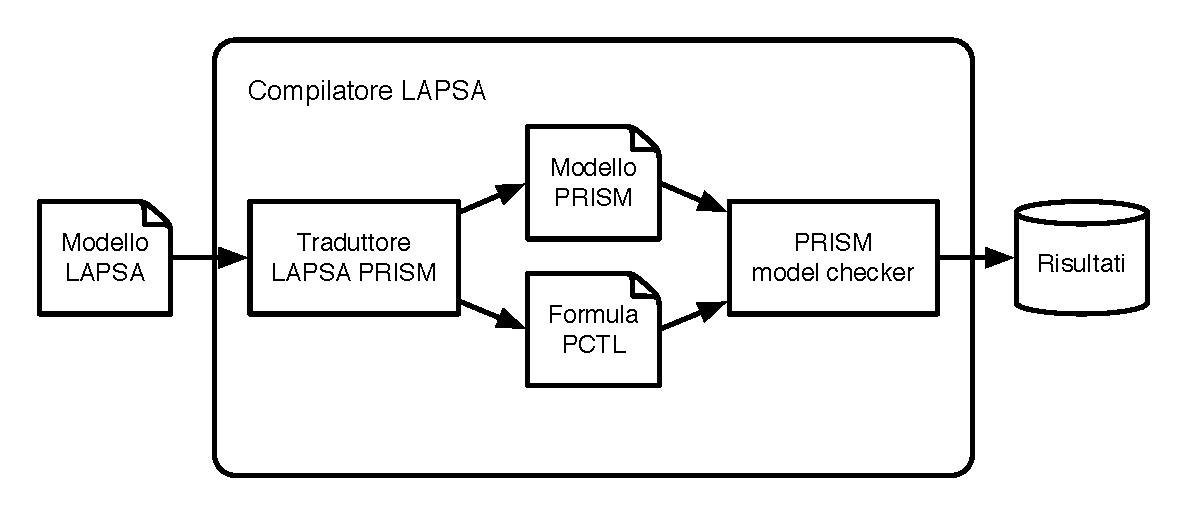
\includegraphics[width=\textwidth]{Images/lapsa}
	\end{centering}
	\caption{Schema del compilatore \ac{lapsa}}
	\label{fig:lapsa:compiler}
\end{figure}

Al fine di migliorare le prestazioni è stato pensato di strutturare i risultati in modo leggermente più complesso:
\begin{verbatim}
	Hashtable<List<Integer>,Hashtable<List<Integer>,Double>> results;
\end{verbatim}
La struttura è quindi una hashtable di hashtable di probabilità. Il primo livello ha come chiave la lista dei parametri che identifica lo stato del modulo principale mentre la seconda è la lista di parametri che identifica lo stato dei moduli che compongono l'ambiente. In questo modo i tempi di lettura rimangono costanti, ma risulta più semplice applicare algoritmi di ricerca del massimo dei minimi: generalmente si procede cercando il caso peggiore che si può verificare nell'ambiente, in termini di probabilità, e si indaga sulla scelta che porta al risultato migliore con una ricerca del massimo.

Come illustrato in figura \ref{img:laspsa:compiler2} il compilatore \ac{lapsa} è stato pensato per effettuare la decisione delle scelte in una fase precedente alla effettiva esecuzione. Durante la fase di compilazione vengono forniti tramite la hashtable tutti i dati necessari per prendere le decisioni sul campo, quindi il software utilizzato dall'agente non dovrà fare altro che accedere ai dati e prendere la scelta desiderata secondo una politica che ovviamente dovrà concordare con quella espressa nel target del modulo \ac{lapsa}.

\begin{figure}[htbp!]
	\begin{centering}
		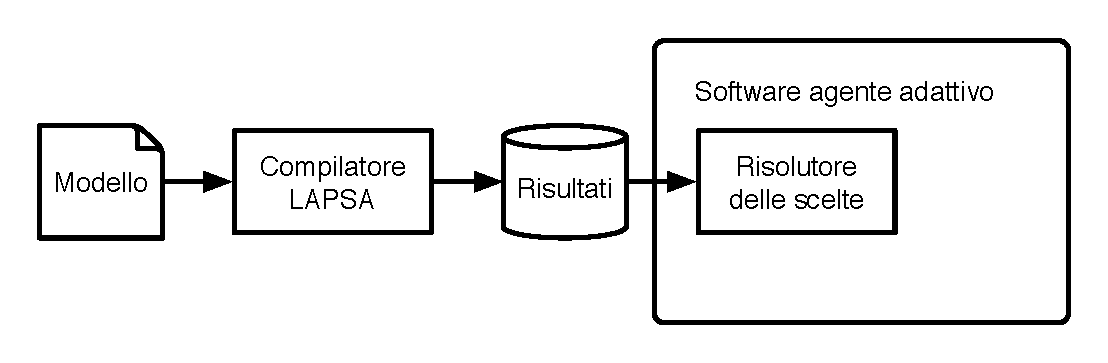
\includegraphics[width=\textwidth]{Images/lapsa2}
	\end{centering}
	\caption{Utilizzo dei risultati nell'agente adattivo}
	\label{fig:lapsa:compiler2}
\end{figure}

Il compilatore del linguaggio \ac{lapsa} è stato implementato tramite il tool \xtext{} \cite{xtext}. Il tool mette a disposizione gli strumenti per definire la grammatica concreta del linguaggio che si vuole tradurre, generando automaticamente tutte le classi \java{} che rappresentano la struttura dei nodi terminali e nonterminali. In questo modo sarà poi possibile implementare il backend facendo riferimento a queste classi ed utilizzandone i metodi visitando l'albero sintattico. La sintassi di \ac{lapsa} è riportata nel listato \ref{code:lapsa:syntax} e segue i costrutti linguistici dati in tabella \ref{tab:lapsaSyntax} ad eccezione di alcune modifiche strettamente legate all'implementazione.

\begin{lstlisting}[language=xtext,style=eclipse,caption={Sintassi di \ac{lapsa} in \xtext{}},label=code:lapsa:syntax]
grammar unifi.marcotinacci.thesis.seal.Seal with org.eclipse.xtext.common.Terminals

import "http://www.eclipse.org/emf/2002/Ecore" as ecore
generate seal "http://www.marcotinacci.unifi/thesis/seal/Seal"

// === main program syntax ===

Program:
	'actions' '{' (actions+=Action)+ '}'
	'subject' modules+=ModuleDefine
	(modules+=ModuleDefine)*
	'environment' ((environment=Environment) | isEmptyEnv?='is empty')
	('ranges' '{' ranges+=Range (',' ranges+=Range)* '}')?
;

Range:
	module=[ModuleDefine] '.' variable=[VariableDeclaration] 'in' '[' from=Value ',' to=Value ']' ('delta' '=' delta=Value)?
;

Action: name=ID ;

// === module syntax ===

ModuleDefine: 
	'module' name=ID '{'
		(variables+=VariableDeclaration ';')+
		(rules+=Rule ';')+
		('target' 'never' never+=Expression)*
	'}'
;

VariableDeclaration:
	type=Type name=ID '=' expr=Expression
;

Type:
	name='int' | name='float' | name='bool'
;

Rule:
	cond=Expression '[' action=[Action] ']' (ndCases+=NDCase)+
;

NDCase:
	'=>' cases+=Case ('#' cases+=Case)*
;

Case:
	'<'weight=Expression (hasCondition?=',' cond=Expression)? '>' update+=Update (',' update+=Update)*
;

Update:
	{ NoAction } 'noaction' | 
	{ Assign } variable=[VariableDeclaration] '=' expr=Expression
;

Environment:
	modules+=[ModuleDefine] ('|{' (actions+=[Action])+ '}|' modules+=[ModuleDefine])*
;


// === expression syntax ===

Expression:
	Logical;

Logical returns Expression:
	Relation
		(({And.left=current} 'and' 
		| {Or.left=current} 'or') 
		right=Relation)*;

Relation returns Expression:
	Addition 
		(({Leq.left=current} '<='
		| {Less.left=current} '<'
		| {Eq.left=current} '=='
		| {Neq.left=current} '!='
		| {Geq.left=current} '>='
		| {Gtr.left=current} '>')
		right=Addition)?;

Addition returns Expression:
	Multiplication 
		(({Plus.left=current} '+' 
		| {Minus.left=current} '-') 
		right=Multiplication)*;

Multiplication returns Expression:
	PrimaryExpression 
		(({Multi.left=current} '*' 
		| {Div.left=current} '/') 
		right=PrimaryExpression)*;

PrimaryExpression returns Expression:
	'(' Expression ')'
	| { Not } 'not' cond=PrimaryExpression
	| { Literal } value=Value
	| { Quantifier } 'exists' name=ID ':' module=[ModuleDefine] 'such that' cond=PrimaryExpression
	| { ExternalReference } module=[Quantifier] '.' variable=[VariableDeclaration] 
	| { LocalReference } ('this' '.')? variable=[VariableDeclaration]   
;

Value: INT | FLOAT | BOOL;

terminal INT returns ecore::EInt: ('0'..'9')+;

terminal FLOAT returns ecore::EDouble:
  ('-')? (INT)* ('.' (INT)+)? |
  ('-')? (INT)+ ('.') | 
  ('-')? (INT)+ ('.' (INT)*)? (('e'|'E')('-'|'+')? (INT)+);

terminal BOOL returns ecore::EBoolean: 'true' | 'false';
\end{lstlisting}

L'implementazione del compilatore avviene attraverso la definizione della funzione \texttt{doGenerate} offerta da \xtext{}. L'implementazione è riportata nel listato \ref{cod:xtend:generate} e consiste nelle fasi principali citate in precedenza: generazione del modello \prism{} e della formula obiettivo \ac{pctl}, esecuzione del model checking ed esportazione dei risultati serializzando la hashtable nel file \texttt{hashtable.ser}.

\begin{lstlisting}[language=xtend,style=eclipse,caption={Implementazione della funzione di generazione in \xtend{}},label=code:xtend:generate]
	override void doGenerate(Resource resource, IFileSystemAccess fsa) {
		modules = new LinkedList<ModuleDefine>
		renaming = new Hashtable<String, Integer>
		moduleCounter = -1

		var Program p = resource.contents.get(0) as Program
		if(p.isEmptyEnv) env = null
		else env = p.environment

		// prism model generation
		fsa.generateFile("model.pm", p.prismCompile)

		// model checking
		var fh = new FormulaHandler(resource)
		
		moduleCounter = 0
		fh.execModelCheck(p.modules.get(0).never.get(0).prismCompileExpression.toString)
		
		// serialize hashmap
        var objOut = new ObjectOutputStream(
        	new FileOutputStream(Commons::getSrcGenURI(resource)+"hashmtable.ser")
        )
        objOut.writeObject(fh.index);
        objOut.close();
	}
\end{lstlisting}

La generazione del modello \prism{} ha inizio a partire dal nodo iniziale \emph{program} e scende fino alle foglie dell'albero sintattico. All'interno del listato \ref{code:xtend:program} vengono mostrate le funzioni che traducono il nodo \emph{program} e i nodi \emph{module} in condice \prism{}. Nel nodo program viene specificato che si tratta di un modello \ac{mdp} e viene data la traduzione del modulo principale e di quelli dell'ambiente, se ce ne sono. Ogni modulo, a sua volta, viene compilato rimandando la traduzione di ogni nodo \emph{variable} e \emph{rule} che contiene. I nomi delle variabili sono gestiti con un valore numerico incrementale (\texttt{moduleCounter}) in modo da non avere ambiguità.

\begin{lstlisting}[language=xtend,style=eclipse,caption={Implementazione della funzione di generazione in \xtend{}},label=code:xtend:program]
	def CharSequence prismCompile(Program p){
		var CharSequence tpl = '''
		mdp
		
		// === MODULES ===
		
		<<p.modules.get(0).prismCompile>>
		'''
		
		if(!p.isEmptyEnv){
			tpl = 
			'''
			<<tpl>>
			<<FOR m:p.environment.modules>>
				<<m.prismCompile>>
			<<ENDFOR>>
			'''
		}
		tpl
	}
		
	def prismCompile(ModuleDefine m){
		moduleCounter=moduleCounter+1
		'''
		module module_<<moduleCounter>>
		// variables
		<<FOR v:m.variables>>
			<<v.prismCompile>>
		<<ENDFOR>>
		// rules
		<<FOR r:m.rules>>
			<<r.prismCompile>>
		<<ENDFOR>>
		endmodule
		'''
	}
\end{lstlisting}

La dichiarazione di variabili viene implementata come descritto nel listato \ref{code:xtend:vars}, recuperando il range dal nodo \emph{ranges} e distinguendo il caso sui tre tipi di variabile che si possono verificare. La variabile booleana ha una mappatura quasi naturale in quanto ci si limita ad aggiungergli solamente la valutazione dell'assegnamento iniziale. Per le variabili intere viene anche specificato il range riportando i valori selezionati. Per gestire le variabili \emph{float} si esegue una discretizzazione: all'interno della sezione \emph{ranges} del file \ac{lapsa} dovranno essere stati specificati i parametri di inizio e fine del dominio e un valore $\delta$ (di default uguale a uno) che specifichi l'ampiezza dell'intervallo di discretizzazione. Il dominio discretizzato viene quindi mappato nel dominio degli interi a partire dallo zero e anche il valore di inizializzazione verrà riadattato allo stesso modo.

\begin{lstlisting}[language=xtend,style=eclipse,caption={Traduzione della dichiarazione di variabili da \ac{lapsa} a \prism{}},label=code:xtend:vars]
	def prismCompile(VariableDeclaration v){
		var from = 0
		var to = 1
		var delta = 1

		// look at ranges and get bounds
		for(r:(v.eContainer.eContainer as Program).ranges){
			if(r.variable==v){
				to = Integer::parseInt(r.to)
				from = Integer::parseInt(r.from)
				if(r.delta != null){
					delta = Integer::parseInt(r.delta)
				}
			}
		}
		'''
		<<v.localName>> : 
		<<IF v.type.name.equals('bool')>>
			bool init <<v.expr.prismCompileExpression>>;
		<<ENDIF>>
		<<IF v.type.name.equals('int')>>
			[<<from>>..<<to>>] init <<v.expr.prismCompileExpression>>;
		<<ENDIF>>
		<<IF v.type.name.equals('float')>>
			[0..floor((<<to>>-<<from>>)/<<delta>>)] init
			ceil((<<v.expr.prismCompileExpression>>-<<from>>)/<<delta>>);
		<<ENDIF>>
		'''
	}
\end{lstlisting}

Come ultima procedura descriviamo la traduzione delle transizioni da \ac{lapsa} a \prism{} (listato \ref{code:xtend:rules}). La condizione di base rappresenta la guardia che abilita la transizione e viene definita una volta inizialmente e riutilizzata se necessario. Può infatti succedere, nel caso in cui utilizziamo il costrutto di scelta nondeterministica, che la condizione debba essere riscritta nel codice \prism{} che non può prevedere quel tipo di espressione. Il primo ciclo scandisce infatti ogni caso nondeterministico e genera una transizione per ciascuno. Il secondo invece si occupa dei casi delle distribuzioni probabilistiche provvisti di guardie generando tutte le combinazioni di condizioni soddisfatte e non. Viene quindi inserita la condizione di base seguita da tutte le condizioni aggiunte dalle dai casi probabilistici provvisti di guardia. Se non ci sono casi allora viene inserita la transizione \emph{true} a probabilità $1$, altrimenti un ulteriore ciclo scandisce i casi presenti. Le probabilità vengono normalizzate in modo che una transizione abbia sempre la distribuzione dei casi a somma $1$, mentre le espressioni di aggiornamento vengono ricavate dai nodi \emph{update}.

\begin{lstlisting}[language=xtend,style=eclipse,caption={Traduzione delle transizioni da \ac{lapsa} a \prism{}},label=code:xtend:rules]
	def prismCompile(Rule r){
		val baseCondition = '''
			[<<r.action.name>>] <<r.cond.prismCompileExpression>>'''
		// add unconditioned cases and true cases
		'''
		<<FOR ndcase:r.ndCases>>
		<<FOR comb:ndcase.cases.reduced.allCombinations 
			SEPARATOR ';' AFTER ';'>>
		<<baseCondition>>
		<<FOR c:ndcase.cases.filter(c|c.hasCondition) 
			BEFORE '&' SEPARATOR '&'>>
			<<IF !comb.contains(c)>>!<<ENDIF>>(<<c.cond.prismCompileExpression>>)
		<<ENDFOR>> 
		-> 
		<<IF comb.size==0 && ndcase.cases.filter(c | !c.hasCondition).size==0>>
			1 : true
		<<ELSE>>
			<<FOR c : ndcase.cases.filter(c | !c.hasCondition 
				|| comb.contains(c)) SEPARATOR '+'>>
				(<<c.weight.prismCompileExpression>>) /
				(<<ndcase.totalWeight(comb)>>) :
				<<FOR u:c.update SEPARATOR '&'>>
					<<u.prismCompileUpdate>>
				<<ENDFOR>>
			<<ENDFOR>>
		<<ENDIF>>
		<<ENDFOR>>
		<<ENDFOR>>
		'''
	}
\end{lstlisting}